% Author: Till Tantau
% Source: The PGF/TikZ manual
\documentclass[a4paper,11pt]{article}
\usepackage[utf8]{inputenc}
\usepackage{listings}
\usepackage{amsmath}    % need for subequations
\usepackage{graphicx}   % need for figures
\usepackage{verbatim}   % useful for program listings
\usepackage{color}      % use if color is used in text
\usepackage{subfigure}  % use for side-by-side figures
\usepackage{hyperref}   % use for hypertext links, including those to external documents and URLs
\usepackage{url}
\usepackage{float}
\usepackage{tikz}
\usepackage{enumitem}
\usepackage{hyperref}
\usepackage{pdfpages}
\usepackage{listings}
\usepackage{color}
\usepackage[T1]{fontenc} % use for allowing < and > in cleartext
\usepackage{fixltx2e}    % use for textsubscript
\newcommand{\BigO}[1]{\ensuremath{\operatorname{O}\left(#1\right)}}

\bibliographystyle{plain}
\begin{document}
\date{1. December 2013}
\title{Bla Bla Bla\\Underblabla}
\author{Marcus Gregersen\and Martin Faartoft\and Rick Marker}
%Overkill med forside / abstract / titel / undertitel?
\clearpage\maketitle
\thispagestyle{empty}
\setcounter{page}{1}
\section{Preface}
\section{Problem 1 - Best buddies}
%Hvad skriver vi her?

\section{Problem 2 - Popular}
\subsection{Introduction}
In this section, we try to answer the question: "How many unique co-actors has a a given actor starred in at least one movie with". We will develop and run a Map-Reduce algorithm using the Hadoop framework, both locally and on the Amazon Elastic Cloud service.
\paragraph{}
To validate and discuss the Map-Reduce implementation, we will create a sequential algorithm that also solves the \emph{Popular} problem. To make the Map-Reduce algorithm more interesting, we have have deliberately projected the IMDB dataset to a text file, in a format where each line contains the id of an actor followed by a list of movie ids, one id for each movie that actor starred in.\footnote{This forces the Map-Reduce algorithm to use 2 rounds of computation.}
\paragraph{} 
To allow for comparison between the sequential and the Map-Reduce algorithms, we have made the sequential algorithm accept the same input.
%TODO skriv noget om problem size, antal actors, antal movies, textfil størrelse
\subsection{Sequential Algorithm}
\label{sub:sequential}
In our sequential algorithm we start by building a reverse index, that maps movies to actors. This allow us to check which actors apperead in which film in constant time. Building this index is done in \BigO{a*m} time, where \emph{a} is the number of actors and \emph{m} is the number of movies\\

When the reverse index is build, we run through all of the actors, and for each actor we run through all the movies they have appeared in, and for all the movies they have appeared in, we note which actors are in those movies. For each actor a given actor has starred with we add it to that actors total. Even though all lookups are implemented to be done in constant time,  having 3 nested loops, we get a running time of \BigO{a^2*m}. In the end we output our data which takes another \BigO{a*m} time.\\

All this gives our sequential algorithm a running time of \BigO{a^2*m}. Even though we have found an upper bound, it is by no means a strict upper bound. If we envision a matrix with actors and movies, where each entry is 1 if the actor appeared in the movie, or empty otherwise, we can see that the matrix is pretty sparse with the given IMDB dataset. As a result the actual running time of our algorithm will be much lower.

\subsection{Map-Reduce Algorithm}
\label{sub:map-reduce}
\begin{figure}
\centering 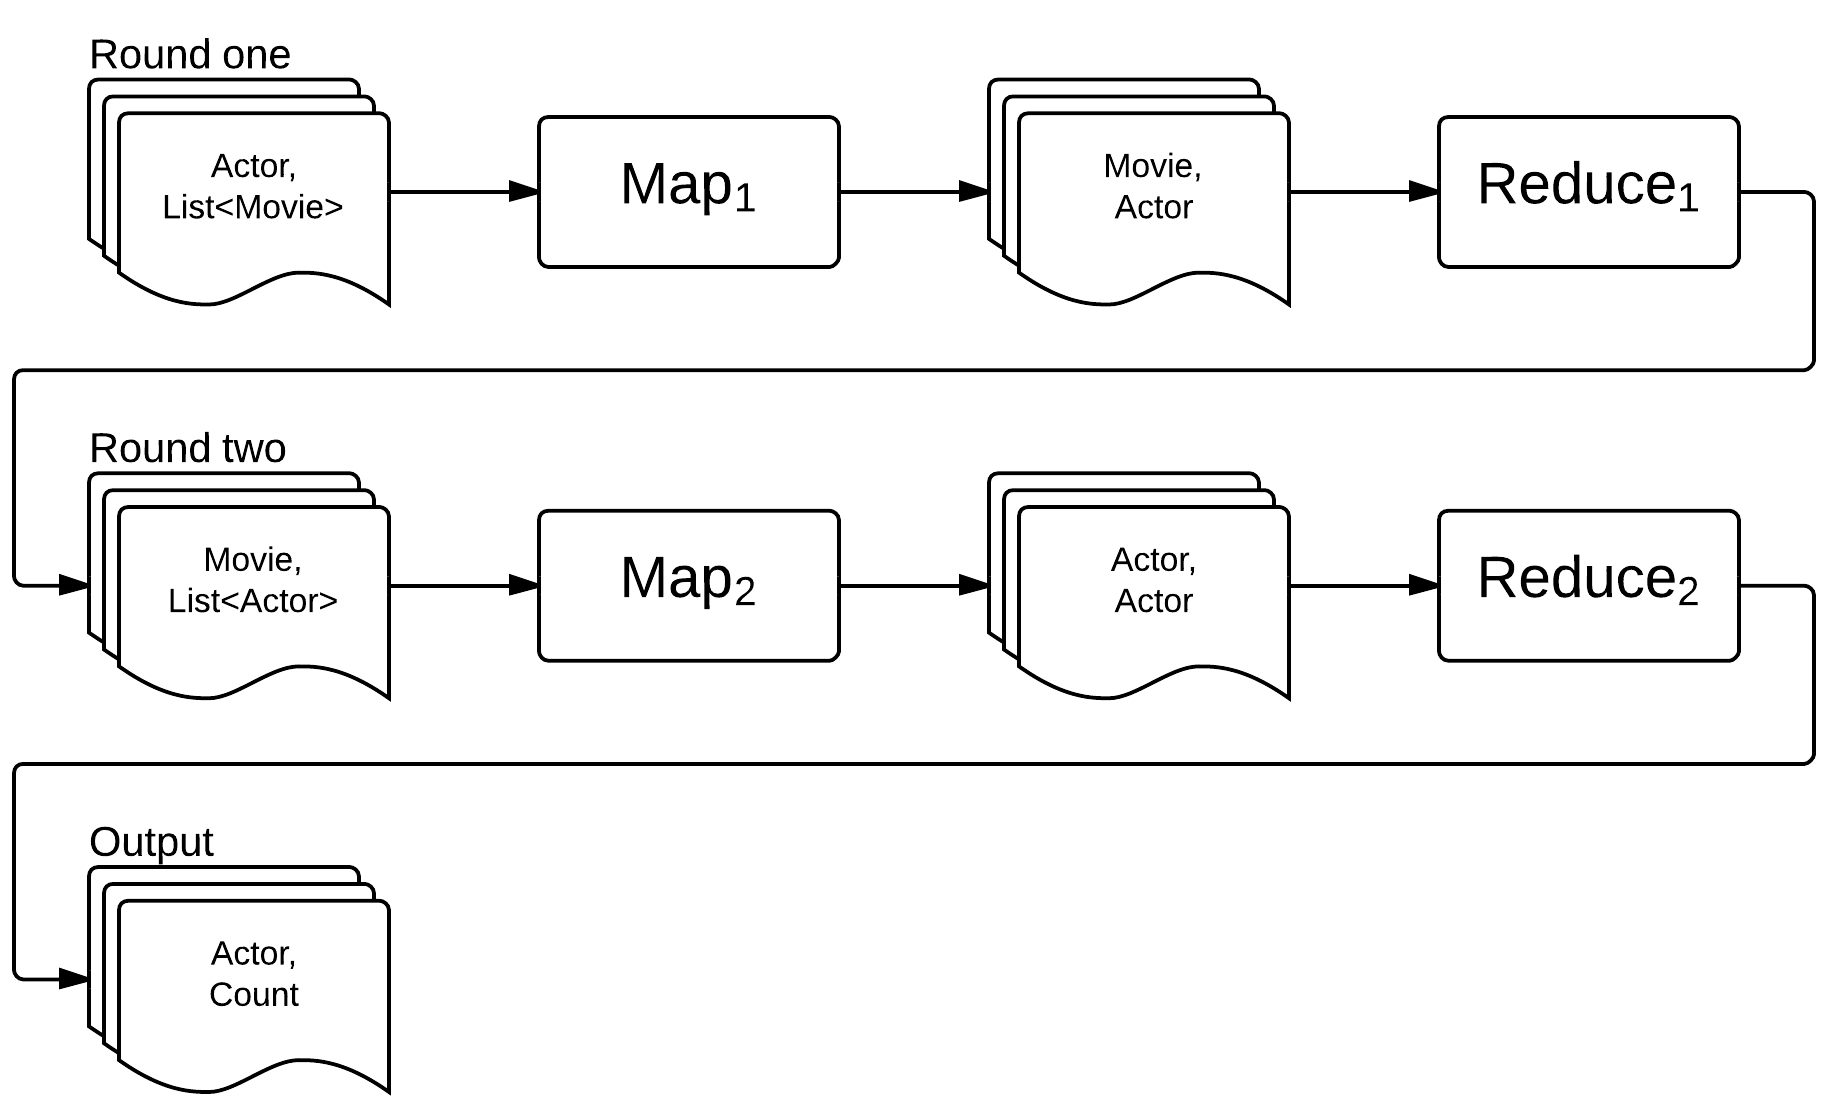
\includegraphics[scale=0.2]{map-reduce-figure.png}
\vspace{-10pt}
\caption{Map-Reduce overview}
\label{fig:map-reduce}
\vspace{-10pt}
\end{figure}

Solving the \emph{Popular} problem using Map-Reduce with the specified input format, requires two rounds. The first round will re-project the original input, while the second round will count the number of unique pairings of actors.

\subsubsection{Round One}
Goal: Transform input pairs (Actor, List<Movie>) into output pairs (Movie, List<Actor>).\\

The mappers break down the (Actor, List<Movie>) pairs into a series of (Movie, Actor) pairs, one for each Movie in the input List<Movie>, essentially saying "this actor played in this movie".\\

The reducers each receive a list of (Movie, Actor) pairs (no reducer receives pairs with different keys), and builds from those a pair of shape (Movie, List<Actor>) by simply appending each actor to a list. The output of round one is thus, a pivot of the input data changing the shape from (Actor, List<Movie>) to (Movie, List<Actor>), essentially saying "this movie contained exactly these actors".

\subsubsection{Round Two}
\label{sub}
Goal: Transform input pairs (Movie, List<Actor>) into output pairs (Actor, Count), where count is the number of unique co-actors this actor has starred with in a movie.\\

The mappers break down the (Movie, List<Actor>) pairs into all possible Actor-pairs along with their inverses.

\begin{verbatim}
function RoundTwoMap(...)
    for(actor a in actors)
        for(actor b in actors)
            if(a != b)
                emit(a, b)
\end{verbatim}

This produces a number of pairs, that is quadratic in the number of actors in the movie, each capturing the information "Actor A played with Actor B in some movie".\\

The reducers each receive a list of (Actor\textsubscript{key}, Actor\textsubscript{value}) pairs, and using a Java HashSet, they filter out any duplicate pairs, and emit the final (Actor, count) pair. These pairs show the number of unique co-actors, a given actor has had during his career.

\subsubsection{Analysis}
To gauge the efficiency of our implementation, we look at three measures. The number of rounds in the computation, the amount of work done in each mapper/reducer in the worst case, and the number of pairs emitted.

\paragraph{Number of rounds}
The algorithm runs in a constant number of rounds (2), independent of the problem size. As mentioned previously, this can be reduced to a single round, if the input has the desired structure.

\paragraph{Skewness of work distribution}
The amount of work done in each mapper/reducer is close to balanced. Obviously, the round two reducer assigned to the most productive actor in the dataset, will do more work than the reducer assigned to an actor that only ever starred in a single movie, but in terms of the input size, these numbers are roughly equal. This is true because no single actor has played in a significant fraction of movies in the dataset.\\
% TODO: Should we expand on "tricks", possibly with a ref
If the dataset was close to being fully connected, additional techniques, beyond the scope of this project, would be needed to balance the workload.

\paragraph{Number of pairs}
The number of pairs generated, is 2 for every unique pair of actors that starred in a movie together (Actor\textsubscript{A}, Actor\textsubscript{B}) and vice versa.\\

This is a large amount of pairs, that we would like to reduce. However, we cannot see how this is possible without relaxing the constraint that a pair of actors should be counted only once. If that constraint is removed, the round two mapper can simply emit a single pair for each actor in a movie (Actor, Movies.Actors.count - 1), meaning that "this actor starred with x other actors in some movie". The reducers could then simply sum all those counts, to get the total.\\
% TODO: Should we analyse the other version as an approximation algorithm for the initial problem.
The relaxed version of round two produces drastically fewer pairs (one pair for each actor, for each movie they starred in), compared to the strict version (two pairs for each unique pair of actors per movie). By making the mapper slightly smarter, the shuffler and reducers do much less work. But the end result answers a slightly different question.\footnote{This optimization captures the same idea as the standard 'Wordcount' optimization example, where the mapper keeps a local dictionary of words and counts, instead of mindlessly emitting (word, 1) pairs.}

\subsection{Verification of results}
We have designed the format of the output of our sequential algorithm, described in Section \ref{sub:sequential}, in such a way that it conforms to the format of the Map-Reduce algorithm described in Section \ref{sub:map-reduce}. 
The output is thus on the form:
\begin{verbatim}
[ 
  (Actor_ID_1, Count_1),
  (Actor_ID_2, Count_2),
  ...
  (Actor_ID_n, Count_n)
]
\end{verbatim}
Since we have no guarantee that the row \texttt{Actor\_ID} is sorted in the output of the Map-Reduce algorithm, we have implemented a simple Python script \texttt{sort\_and\_expand.py}. 
The role of this script is firstly to sort the input by \texttt{Actor\_ID} and secondly to add the first and last name of any given actor, for a more humanly readable output.

Having three different outputs produced by a: the sequential algorithm, b: the Map-Reduce algorithm run on a local setup and
c: the Map-Reduce algorithm run on the Amazon Elastic MapReduce service, we then transform each of these outputs using the script.
Using the UNIX tool \texttt{diff}, whose job it is to output the difference between two files, we see that that all three outputs are exactly the same. The fact that the Map-Reduce algorithm produces the exact same output as the independently developed sequential algorithm, gives us a high degree of confidence, that both implementations are correct. The odds of making the same systematic error in both implementations (different programmers, different programming languages, different algorithmic paradigms) are very small.

The first 10 lines of the output, i.e the top 10 actors that has starred with most unique actors are: 
\begin{verbatim}
(621468, 'Bess Flowers', 10834)
(372839, 'Lee Phelps', 6679)
(74450, 'John Carradine', 6447)
(212581, 'Stuart Holmes', 6318)
(152868, 'James Flavin', 6027)
(22585, 'Irving Bacon', 5957)
(233082, 'James Earl Jones', 5894)
(245158, 'Donald (I) Kerr', 5775)
(209799, 'Adolf Hitler', 5773)
(433904, 'Martin Sheen', 5764)
\end{verbatim}

Taking two samples from the output we see from Bess Flowers' Wikipedia that she was a Hollywood extra that has appeared in over 700 movies. Maybe it is safe to assume that since she has starred in so many movies 

We realize that this is not a formal proof that our result is correct






%MABG
\subsection{Benchmark}

\section{Appendix}

\end{document}
